%%%%%%%%%%%%%%%%%%%%%%%%%%%%%%%%%%%%%%%%%%
%%%%%%%%%%%%%                 %%%%%%%%%%%%
%%%%%%%%%%%%%    EXERCISE 1   %%%%%%%%%%%%
%%%%%%%%%%%%%                 %%%%%%%%%%%%
%%%%%%%%%%%%%%%%%%%%%%%%%%%%%%%%%%%%%%%%%%
\begin{exercise}[]{Given a integer set S, which has n elements in it, you need to divide this set into 2 subarray, where the subarray S1 has m elements, and the subarray S2 has (n-m) elements. the target is minimizing $abs(sum(S1) -sum(S2))$.
    
    Implement your algorithm with C/C++/Python. Please attach your source code named as {\color{red}\emph{Code-P1.*}}. The file \texttt{Data-P1.txt} is a test case, includes an 1-D array of integer with random length, and your program needs to output the final sum. You need to briefly describe your algorithm and find the final sum of \texttt{Data-P1.txt} by your program.
    
    \textbf{Example:} Given input array: $arr[]={1, 6, 11, 5}$. The algorithm should return $1$. The subset $S1=[1, 5, 6], S2=[11]$ .
    }
  \begin{solution}
  \par{~}
  Note that there exist negative inputs in the given testcase. To deal with negative numbers, note that we can take absolute values on the inputs and the result won't change, since we can always move negative number from one set to the other and change its symbol without affecting the output difference.

  With such preprocessing, the problem is reduced to finding a combination of the elements that best approximates half of the sum of all numbers. We can use the idea of knapsack problem to solve this problem.

  For implementation, we try to use the bottom-up dynamic programming to solve the knapsack problem. However, the traditional 2d array is too large for the program to store ($O(S^2)$, where $S$ is the total sum of all inputs). Instead, since the update only uses the previous row of results, we can use $O(S)$ space by maintaining two 1d arrays.

  \begin{algorithm}[H]
    \KwIn{Array $S$ with $n$ integers}
    \KwOut{The minimal $|sum(S_1) - sum(S_2)|$ value, where $(S_1,S_2)$ is a partition of $S$}
    \BlankLine
    Take the absolute value of $S$ \;
    $sum = \sum_i S_i$\;
    $goal = \frac{1}{2} sum$ \;
    Initialize array $now[goal+1]$ and $prev[goal+1]$\;
    \For{$i=0:n-1$}{
      \For{$w=0:goal$}{
        \eIf{$S[i] > w$}{
          $now[w] = prev[w]$\; 
        }{
          $now[w] = \max(prev[w], s[i]+prev[w-s[i]])$\;
        }
      }
      Copy all elements of $now$ into $prev$\;
    }
    \Return{$prev[goal]$}
    \caption{Divide Integer Set \label{js1}}
  \end{algorithm}

  The final result of \texttt{Data-P1.txt} is 1.
  \end{solution}
  \label{ex1}
\end{exercise}



%%%%%%%%%%%%%%%%%%%%%%%%%%%%%%%%%%%%%%%%%%
%%%%%%%%%%%%%                 %%%%%%%%%%%%
%%%%%%%%%%%%%    EXERCISE 2   %%%%%%%%%%%%
%%%%%%%%%%%%%                 %%%%%%%%%%%%
%%%%%%%%%%%%%%%%%%%%%%%%%%%%%%%%%%%%%%%%%%
\begin{exercise}[Bookshelf]{Tim has $n$ books and he wants to make a bookshelf to them. The pages' width of the $i$-th book is $w_i$ and the thickness is $t_i$. 

    Tim puts the books on the bookshelf in the following way. He selects some books and put them vertically. Then the rest of the books are put horizontally above the vertical books. Obviously, the total thickness of the books put vertically must be greater than the sum of widths of the horizontal books. As long as tim wants to make the bookshelf as small as possible, please help him to find the minimum total thickness of the vertical books.

    To simplify the problem, the thickness of each book is either $1$ or $2$. And all the numbers in this problem are positive integers.

    Design an algorithm based on dynamic programming and implement it in C/C++/Python. The file \texttt{Data-P2.txt} is a test case, where the first line contains an integer $n$. Each of the next $n$ lines contains two integers $t_i$ and $w_i$ denoting two attributes of the $i$-th book. Source code should be named as
    {\color{red}\emph{Code-P2.*}} .You need to briefly describe your algorithm and find the result of \texttt{Data-P2.txt} by your program.

    \textbf{Example:} Given $n=5$ books, and $\{(t_i,w_i)|1\leq i \leq 5\} = \{(1,12),(1,3),(2,15),(2,5),(2,1)\}$. The algorithm should return $5$.
}
  \begin{solution}
  \par{~}
  We use dynamic programming to solve this problem. Let $OPT(i,j)$ denotes the minimal sum of the width of the horizontally placed books when the first $i$ books have been placed and the sum of the thickness of the vertically placed books should be limited under $j$.

  Since all books are either of the thickness of 1 or 2, we can ensure the problem will be solved within $O(n^2)$ space. For a new incoming book $i=0,\ldots,n-1$, it will either be placed vertically or horizontally. If placed vertically, $OPT(i,j) =OPT(i-1,j-t_{i-1})$, which is only feasible when $j - t_{i-1} \ge 0$. If placed horizontally, $OPT(i,j) = OPT(i-1,j) + w_{i-1}$.
  
  Note that when building the dynamic programming table, we are not restricting the condition that the total horizontal width should not exceed the total vertical thickness. The constraint will be satisfied when finding the solution. $ans = \min \left\{i | dp[n][i] \le i \right\}$, which holds true by definition of the dp table.

  The implementation can be found in the code, and the result for \texttt{Data-P2.txt} is 2542.

  \end{solution}
  \label{ex2}
\end{exercise}


%%%%%%%%%%%%%%%%%%%%%%%%%%%%%%%%%%%%%%%%%%
%%%%%%%%%%%%%                 %%%%%%%%%%%%
%%%%%%%%%%%%%    EXERCISE 3   %%%%%%%%%%%%
%%%%%%%%%%%%%                 %%%%%%%%%%%%
%%%%%%%%%%%%%%%%%%%%%%%%%%%%%%%%%%%%%%%%%%
\begin{exercise}[String Similarity]{Recall the \emph{String Similarity} problem in class, in which we calculate the edit distance between two strings in a sequence alignment manner.

    You are to find the lowest aligning cost between 2 DNA sequences, in which the cost matrix is defined as

    \begin{center}
        \begin{tabular}{|c||c|c|c|c|c|}
        \hline
          & - & A & T & G & C \\
        \hline
        - & 0 & 1 & 2 & 1 & 3 \\
        A & 1 & 0 & 1 & 5 & 1 \\
        T & 2 & 1 & 0 & 9 & 1 \\
        G & 1 & 5 & 9 & 0 & 1 \\
        C & 3 & 1 & 1 & 1 & 0 \\
        \hline
        \end{tabular}
    \end{center}

    where \texttt{(-, A)} means adding (or removing) one \texttt{A}, etc.

    \begin{enumerate}
        \item
        Implement Hirschberg's algorithm with C/C++/Python. Please attach your source code named as {\color{red}\emph{Code-P3.*}}. Your program will be tested against random inputs. Your program should be able to output two sequences after editing.

        \item
        Using your program, find the edit distance between the two DNA sequences found in attachments \texttt{Data-P3a.txt} and \texttt{Data-P3b.txt}.
    \end{enumerate}}
  \begin{solution}
  \par{~}

  Following the pseudo-code in Figure \ref{fig:ex4} on the textbook, I implemented the DNA edit algorithm. Here are some explanations for the codes.

  \begin{figure}
    \centering
    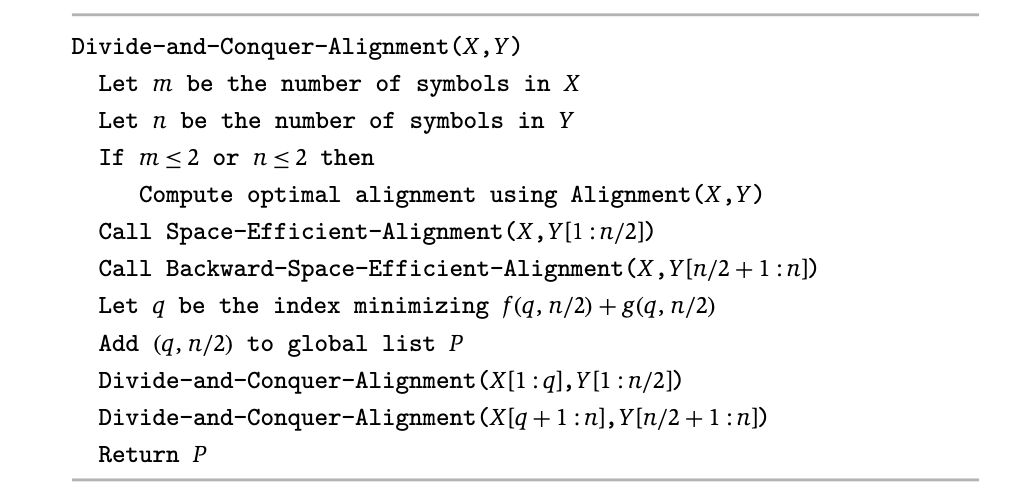
\includegraphics[width=12cm]{img/ex3-1.png}
    \caption{Divide And Conquer Sequence Alignment Algorithm \label{fig:ex4}}
  \end{figure}

  \begin{itemize}
    \item \texttt{vector<pair<int,int> > simpleAlignment(int beg1, int end1, int beg2, int end2)} will use the traditional $O(mn)$ space sequence alignment algorithm, which will be used to deal with the base case in the divide and conquer implementation. The return value is a list of index pairs, starting from \texttt{(beg1, beg2)}, every proceeding item will increase 1 in either or both elements in the pair. The end of the path, namely $\texttt{(end1, end2)}$ won't be in the returned list. The list is used to represent the recovering strategy of the solution. 
    \item \texttt{pair<string, string> originalAlignment(int beg1, int end1, int beg2, int end2)} is the traditional $O(mn)$ space sequence alignment algorithm with solution recovering implemented. It is  written to test the correctness of the divide and conquer implementation.
    \item \texttt{vector<int> spaceEfficientAlignment(int beg1, int end1, int beg2, int end2)} will do space efficient dynamic programming and return the last column of the table for divide and conquer algorithm's use. The values are painted red in Figure \ref{fig:ex5}.
    \item \texttt{vector<int> backwardSpaceEfficientAlignment(int beg1, int end1, int beg2, int end2)} will do reverse space efficient dynamic programming and return the last column of the table for divide and conquer algorithm's use. The values are painted red in Figure \ref{fig:ex5}, which coincide with the positions returned by \texttt{spaceEfficientAlignment}.
    \item \texttt{vector<pair<int,int> > divideAndConquerAlignment(int beg1, int end1, int beg2, int end2)} is the implementation of the algorithm shown in Figure \ref{fig:ex4}. However, the setting of \texttt{q} and the division of the subproblem is slightly different from what is described in the figure. An explanation can be found at \ref{fig:ex5}. In order to concat the path together, $X[q]$ and $Y[n/2]$ will be included in both sub-problems.
  \end{itemize}
  \begin{figure}
    \centering
    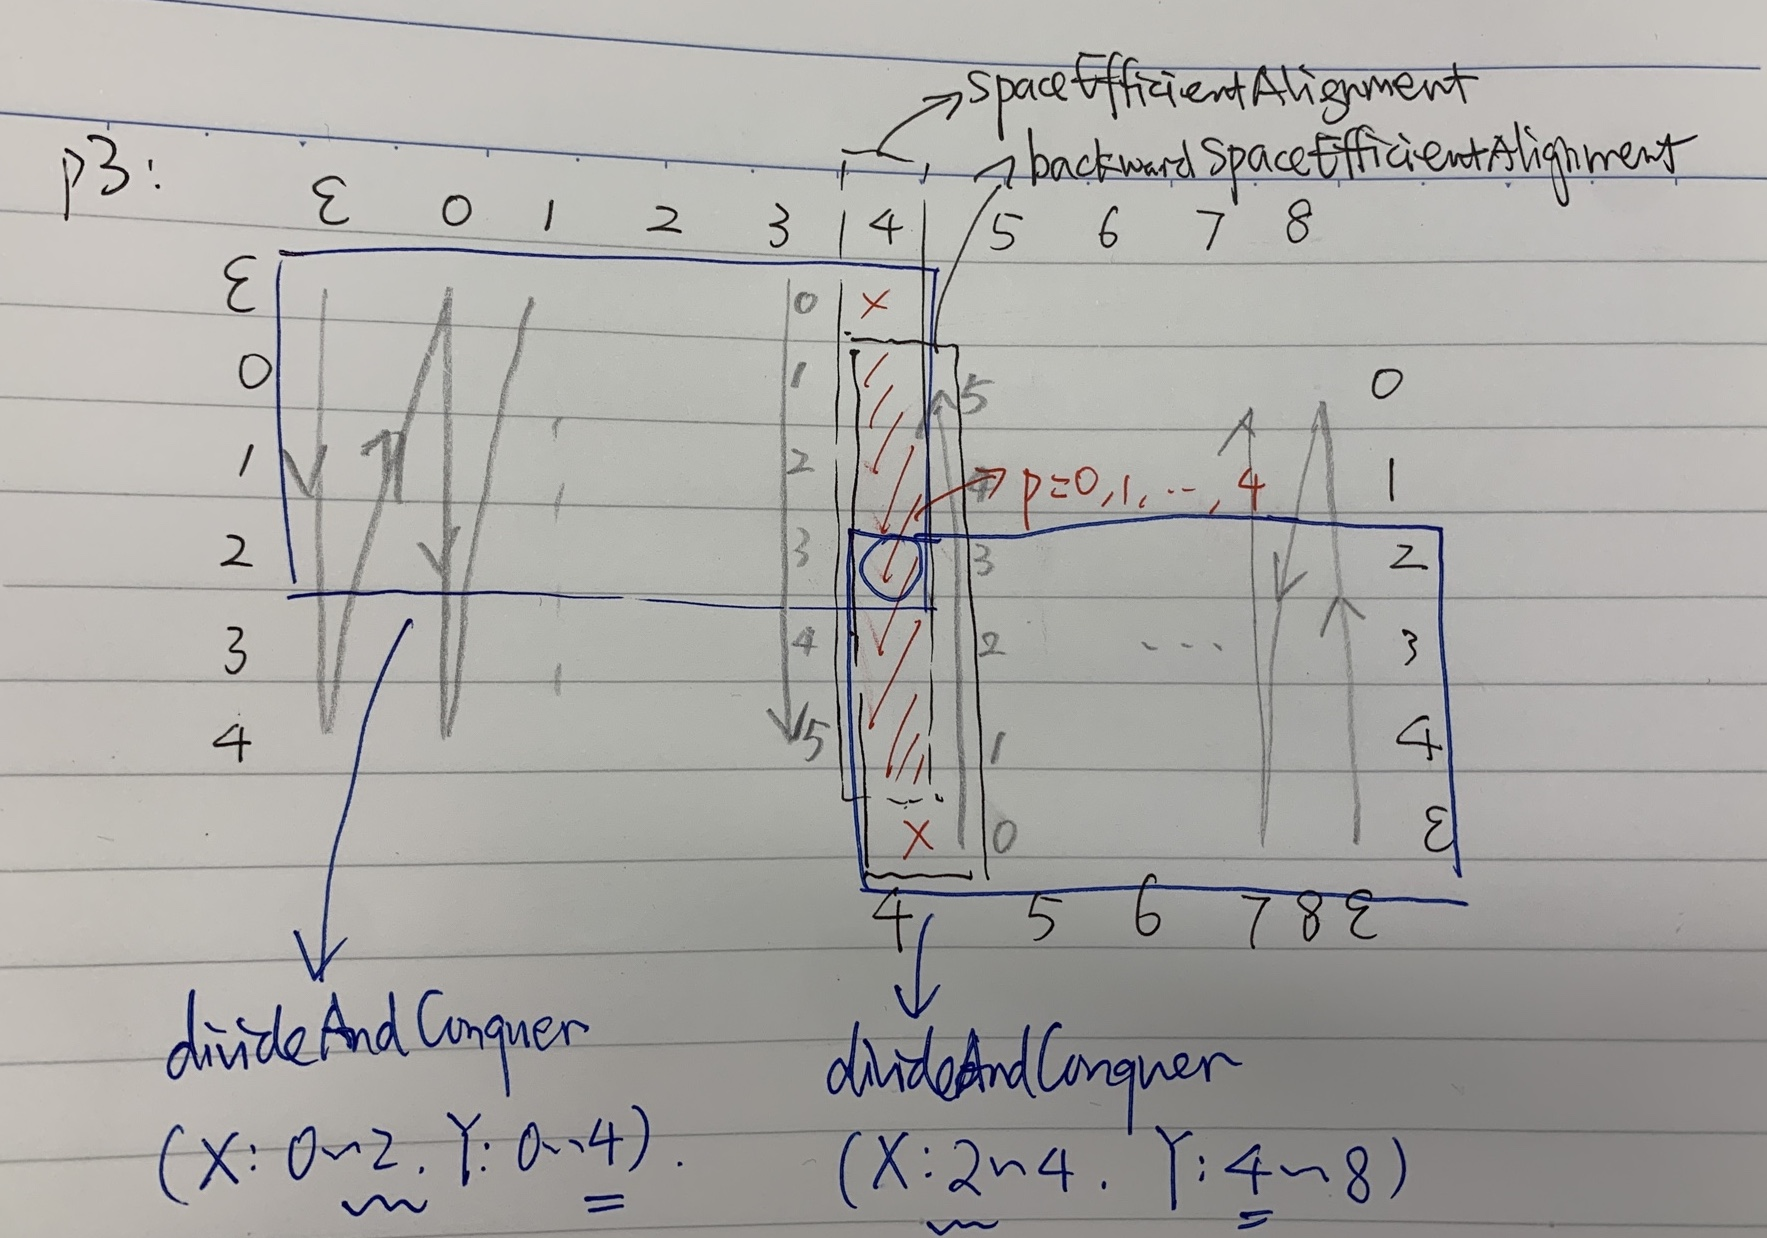
\includegraphics[width=12cm]{img/ex4-2.jpeg}
    \caption{Explanation of my implementation \label{fig:ex5}}
  \end{figure}

  The implementation can be found in the code, and the edit distance for \texttt{Data-P3a.txt} and \texttt{Data-P3b.txt} is 7615. The sequences after editing can be found at \texttt{Ans-P3a.txt} and \texttt{Ans-P3b.txt}.

  \end{solution}
  \label{ex3}
\end{exercise}



%%%%%%%%%%%%%%%%%%%%%%%%%%%%%%%%%%%%%%%%%%
%%%%%%%%%%%%%                 %%%%%%%%%%%%
%%%%%%%%%%%%%    EXERCISE 4   %%%%%%%%%%%%
%%%%%%%%%%%%%                 %%%%%%%%%%%%
%%%%%%%%%%%%%%%%%%%%%%%%%%%%%%%%%%%%%%%%%%
\begin{exercise}[]{Considering you are playing a game with your friend, there are n coins placed in one row with the value of v1, v2, ..., vn, respectively. You and your friend can take one coin from row head or row tail sequentially. If you are the first to choose the coin, write an algorithm to ensure that you can get the maximum profit. Suppose that your friend is as smart as you. 
    ~\\
    Implement your algorithm with C/C++/Python. Please attach your souce code named as {\color{red}\emph{Code-P4.*}}. The file \texttt{Data-P4.txt} is a test case, includes an 1-D array of unsigned integer with random length, and your program needs to output the the coin value list that you choose, and the maximum profit you will get. You need to briefly describe your algorithm and find the final answer of \texttt{Data-P4.txt} by your program.
    
    \textbf{Example:} Given input array: $arr[]={8, 15, 3, 7}$. The algorithm should return your choice list [7, 15], and the final profit 22. 
    
}
  \begin{solution}
  \par{~}

  Note that the game itself can be solved based on the derivation of the sub-optimal structure. We use dynamic programming to solve the problem. Let $OPT(i,j)$ be the return value of the optimal strategy given the array $v_i,v_{i+1},\ldots,v_{j}$.

  Then the recursive derivation of the problem can be depicted as Figure \ref{fig:ex1} shows, with the notion that the opponent wants to minimize the player's return and that the player wants to maximize the return.

  \begin{figure}
    \centering
    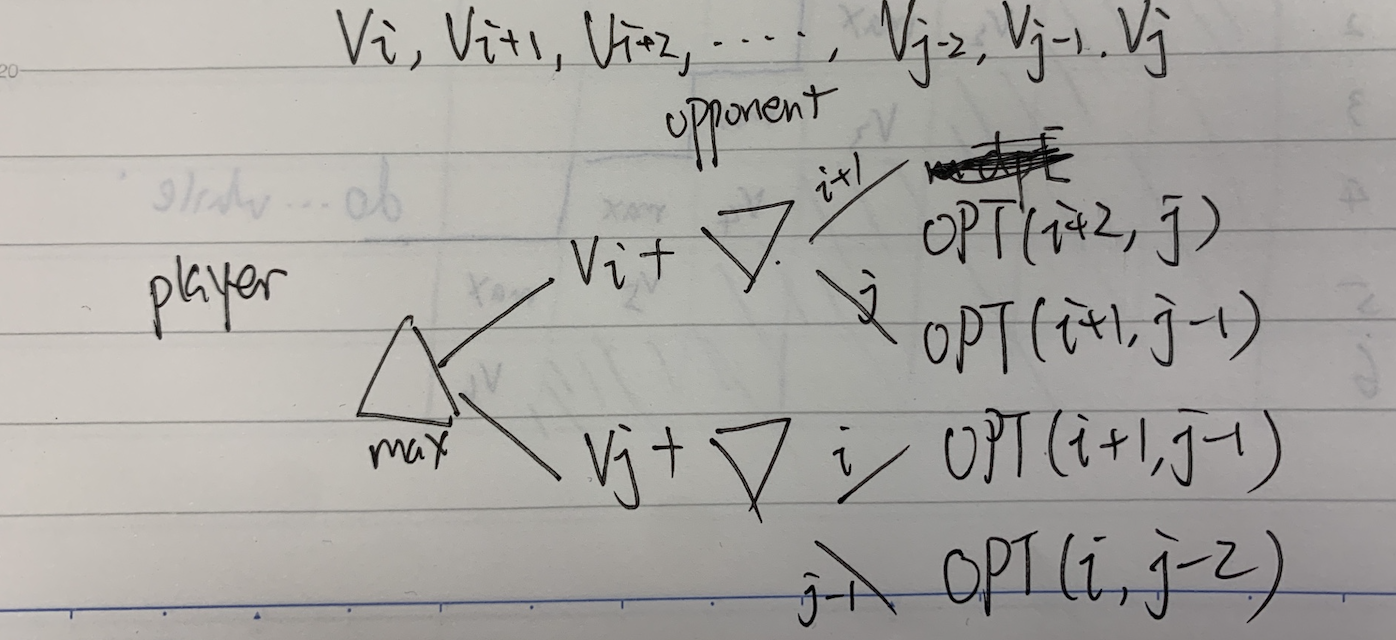
\includegraphics[width=10cm]{img/ex4-1.png}
    \caption{OPT relation\label{fig:ex1}}
  \end{figure}


  As for implementation, the DP table can be constructed as the following picture shows in a bottom-up manner, shown in Figure \ref{fig:ex2}.
  
  \begin{figure}
    \centering
    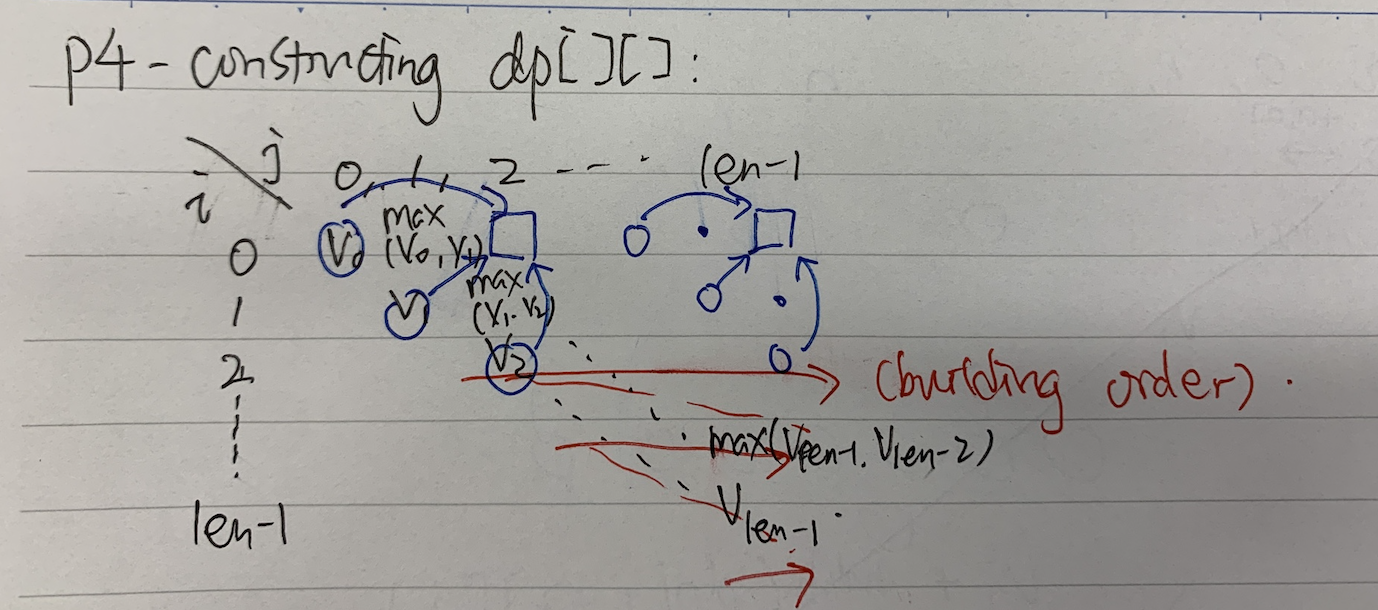
\includegraphics[width=10cm]{img/ex4-2.png}
    \caption{Bottom-up implementation of Dynamic Programming\label{fig:ex2}}
  \end{figure}
  
  The solution recovering can be implemented by backtracking the DP-table, shown in Figure \ref{fig:ex3}.

  \begin{figure}
    \centering
    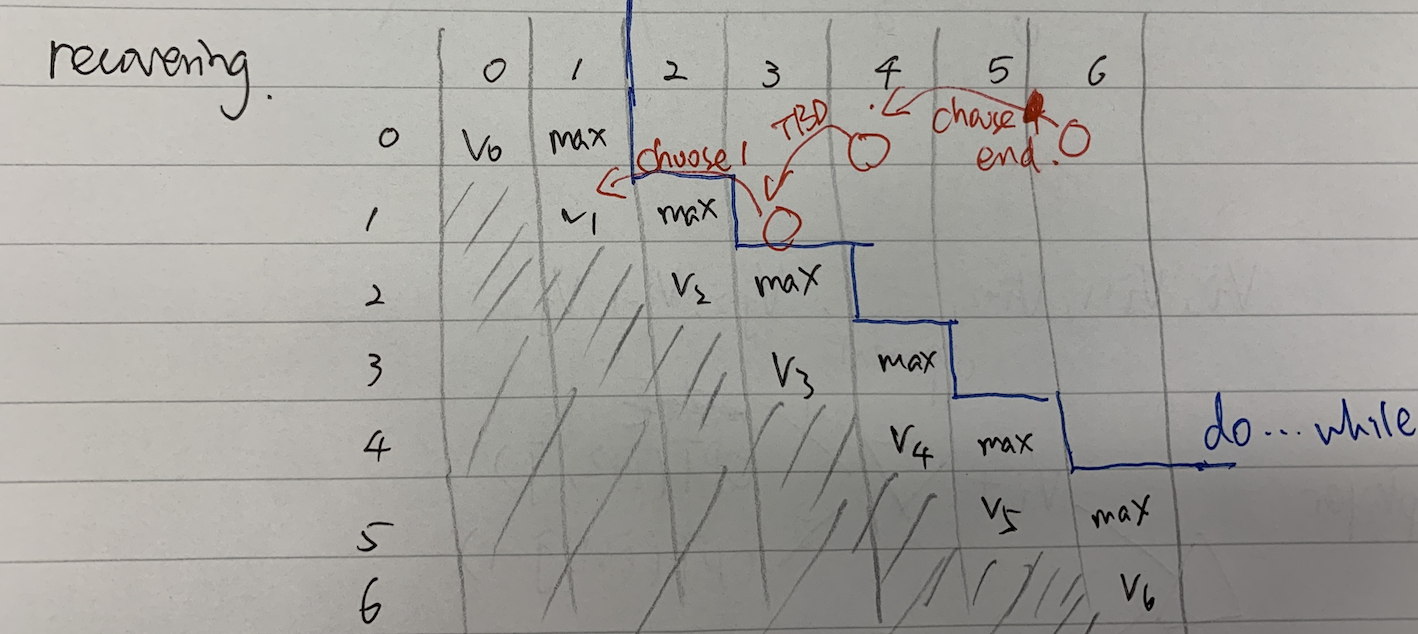
\includegraphics[width=10cm]{img/ex4-3.png}
    \caption{Solution Recover\label{fig:ex3}}
  \end{figure}

  The answer to the input of \texttt{Data-P4.txt} is 250072, and the recovered solution can be found at \texttt{Ans-P4.txt}.

  \end{solution}
  \label{ex4}
\end{exercise}